\documentclass{article}
\usepackage[utf8]{inputenc}
\usepackage[hungarian]{babel}


\usepackage{lipsum}
\usepackage{graphicx} % for the includegrapichs
\usepackage{titling}

\usepackage{fancyhdr} % for the header on the first page
\usepackage{pdfpages} % to include pdf
\usepackage{structuralanalysis} % for the figures
\usepackage{tikz-dimline}
\usepackage{wasysym}

\usepackage{multicol}
\usepackage{amsmath}
\usepackage{t1enc}



\begin{document}
	
	\begin{titlepage}
		\setlength{\headheight}{20pt}
		\lhead{
\includegraphics[height=1.5cm]{logo_mm.png}}
		\rhead{\large{\textbf{Végeselem módszer alapjai}}\\
			BMEGEMMAGMV}
		%\vspace{15cm}
		\title{\huge Kötelező házi feladat 2
		}
		\author{Tar Dániel\\GUTOY7}
		\date{\today}
		\maketitle
		\pagenumbering{gobble}
		\thispagestyle{fancy}
		
		\begin{figure}
			\begin{center}
				
\includegraphics[height=2cm]{logo_bme_kicsi.eps}
			\end{center}
		\end{figure}
		
	\end{titlepage}
	\newpage

	%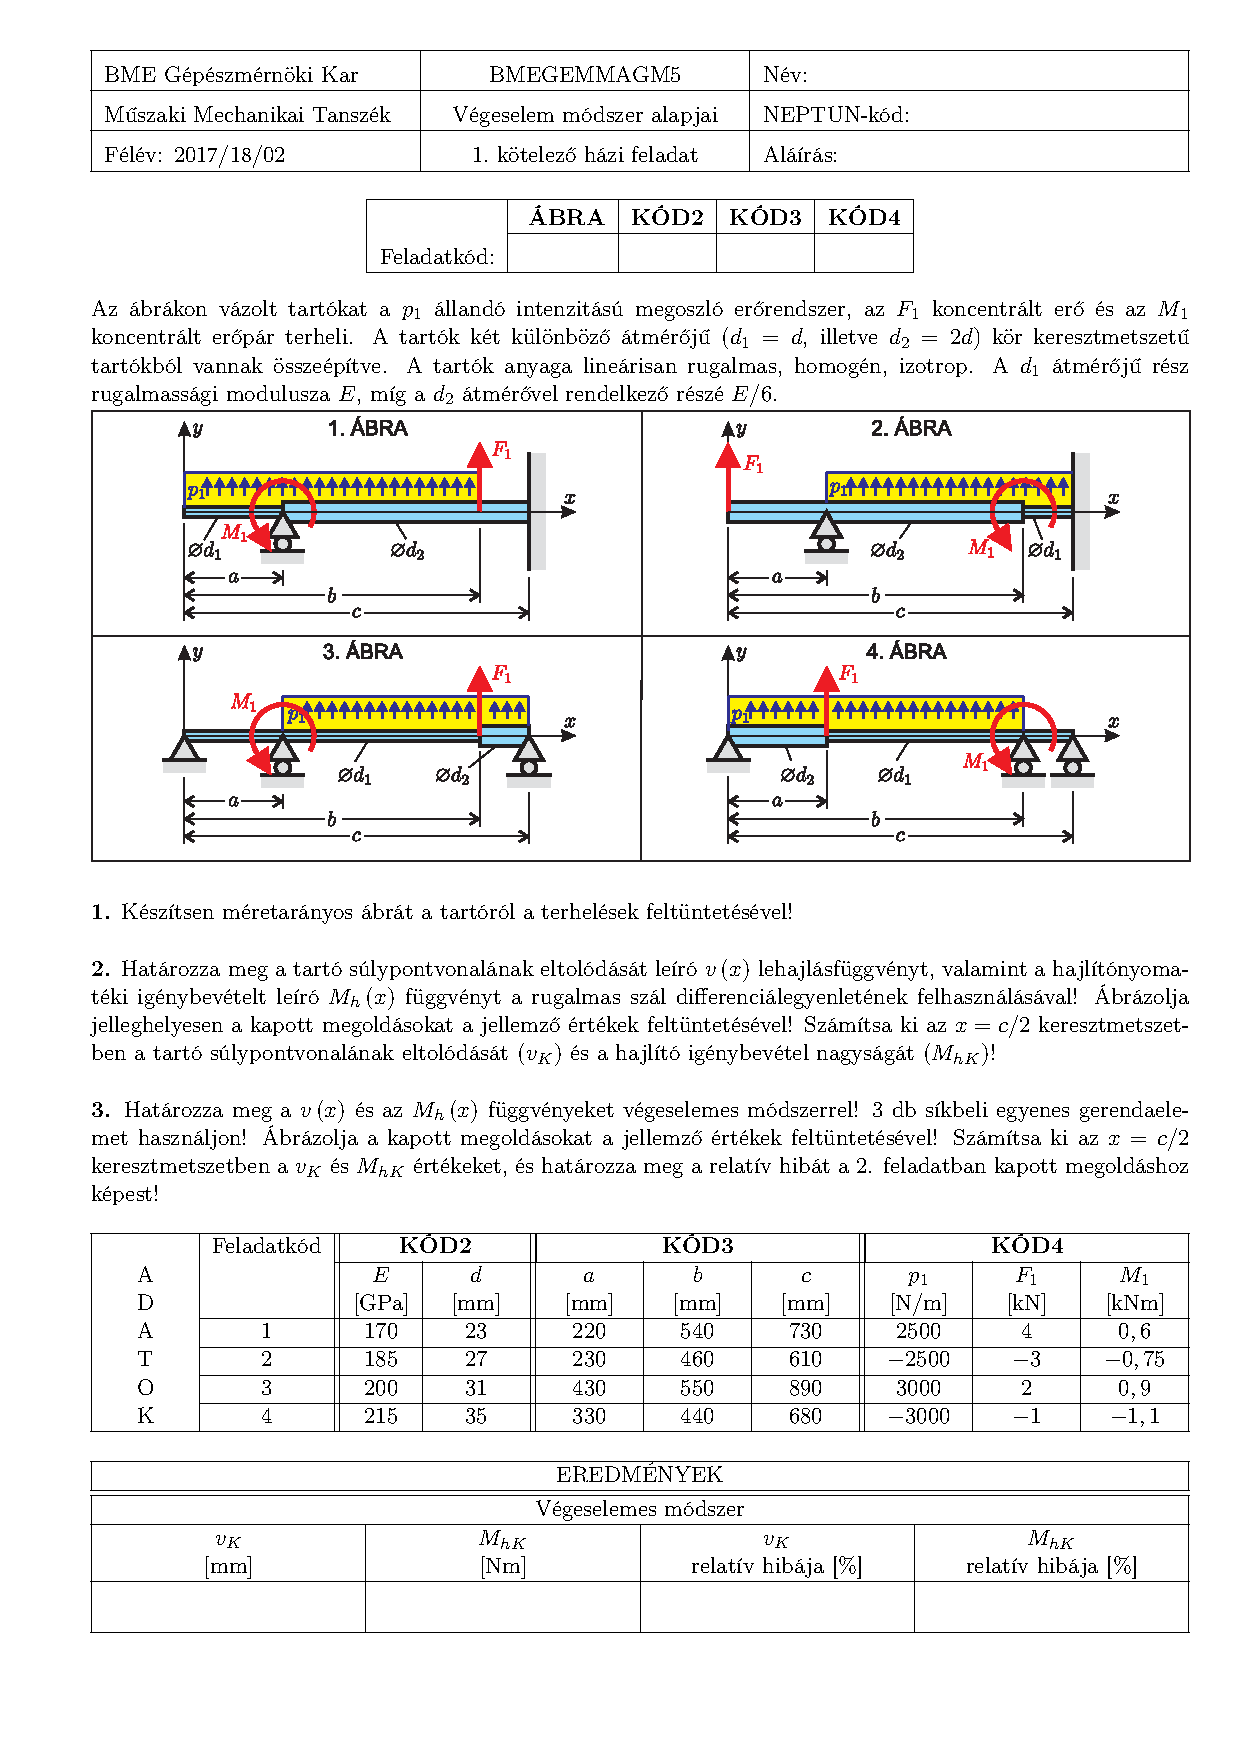
\includepdf{vemalaphf1.pdf}
	 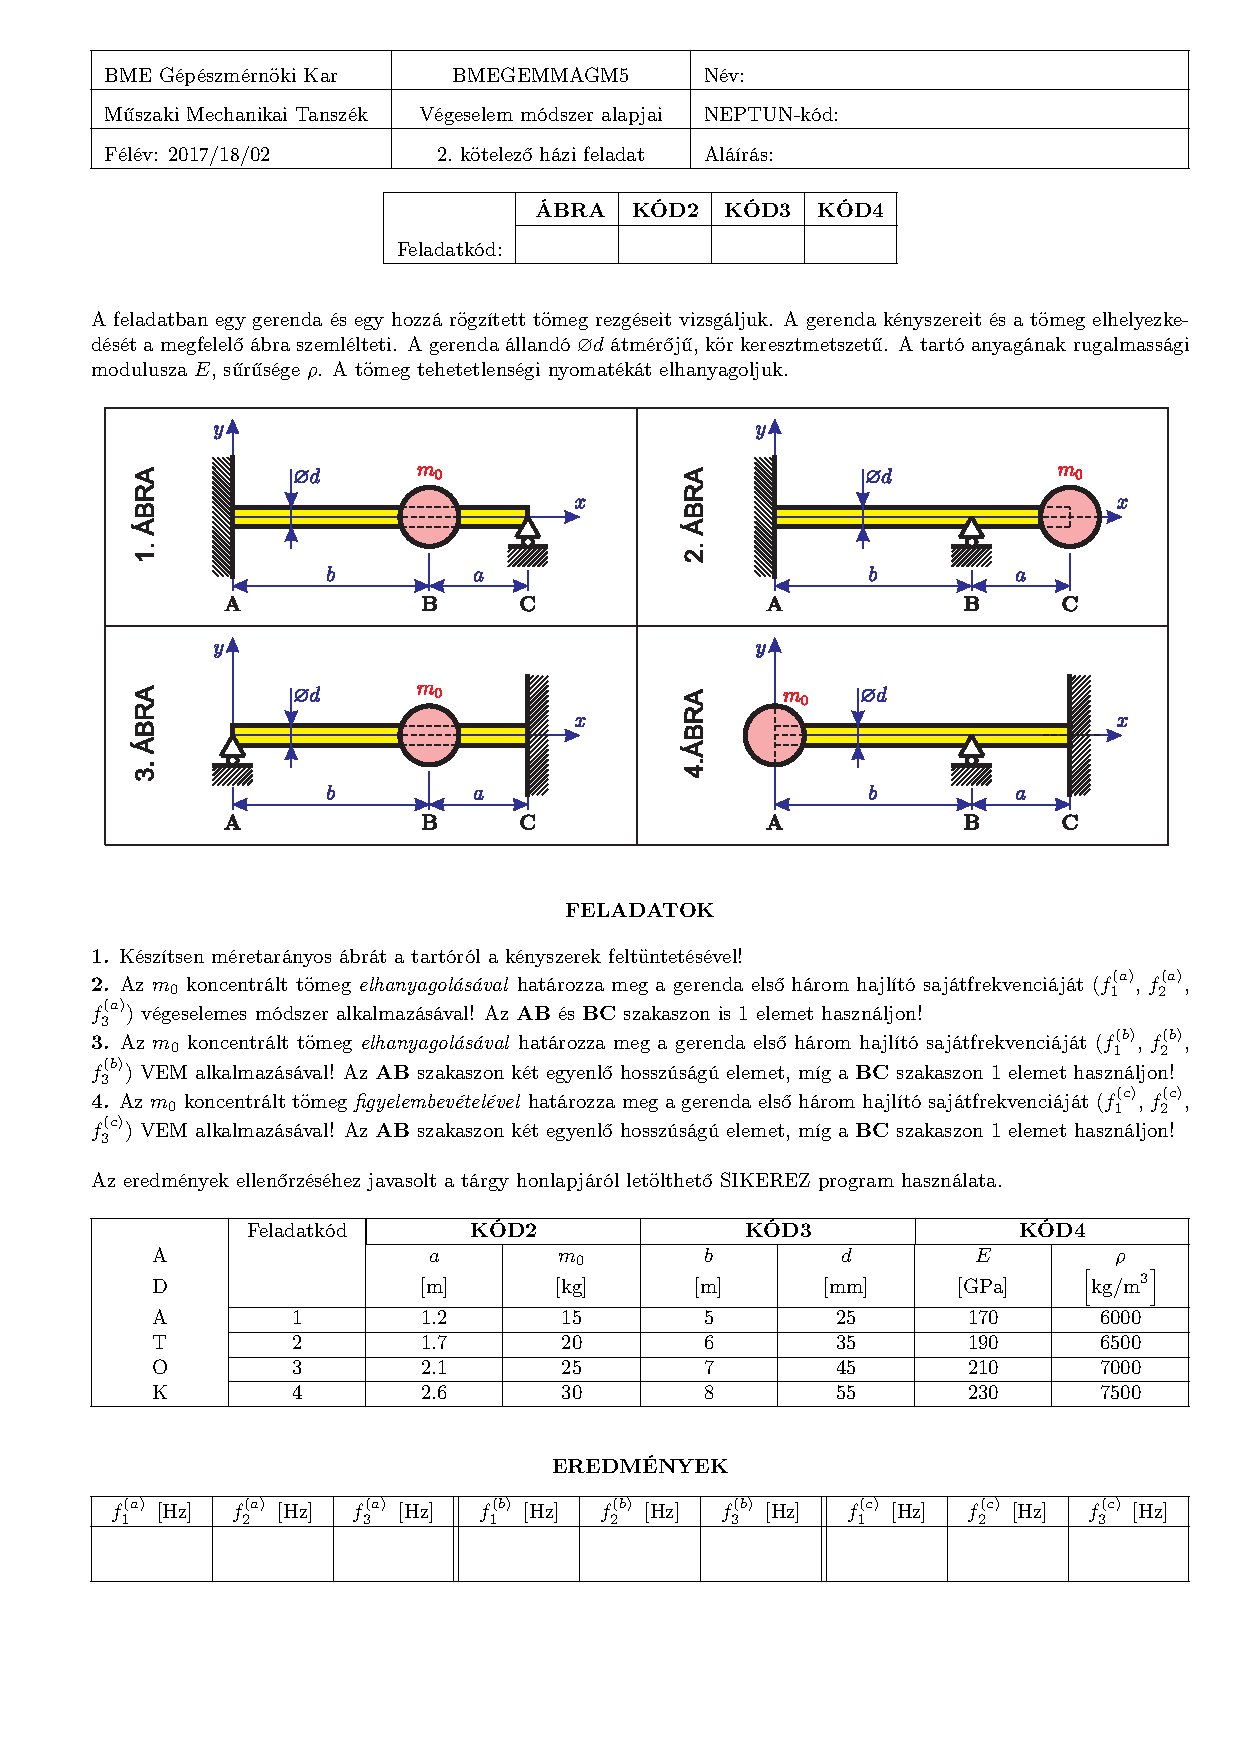
\includepdf[picturecommand*={
	    	\put(460,759){Tar Dániel}
	    	\put(460,742){GUTOY7}
	    	\put(280,680){2}
	    	\put(325,680){1}
	    	\put(368,680){2}
	    	\put(410,680){2}
	    	\put(115,63){eredmeny1}
	    	\put(245,63){eredmeny2}
	    	\put(370,63){eredmeny3}
	    	\put(490,63){eredmeny4}
	 }]{vemalaphf4.pdf}
	\newpage
	
	
	\setlength{\headheight}{0pt}
	\tableofcontents
	\newpage
	
	\pagenumbering{arabic}	
	\setcounter{page}{1}

	
	
	

	
	%\newpage
	
	%---------------------
	% 1.feladat
	%---------------------
	\section{Feladat}
	
	A házifeladat kód alapján az adatok SI mértékegységrendszerben:
	\def\arraystretch{1.2}%
	\begin{table}[h!]
		\begin{center}
			\caption{Adatok}
			\label{tab:table1}
			\begin{tabular}{c|c|c|c|c|c} % <-- Alignments: 1st column left, 2nd middle and 3rd right, with vertical lines in between
				$a$ & $m_{0}$ & $b$ & $d$ & $E$ & $\rho$\\
				$[m]$ & $[kg]$ & $[m]$ & $[m]$ & $[Pa]$ & $[kg/m^{3}]$\\
				\hline
				1,2 & 15 & 6 & 35 & $190\cdot10^3$ & 6500\\
				%2 & 10.1 & b\\
				%3 & 23.113231 & c\\
			\end{tabular}
		\end{center}
	\end{table}
	\def\arraystretch{1}%
	
	Továbbá a rúd keresztmetszetének a felülete:
	\begin{equation}
	A=\frac{d^{2}\cdot\pi}{4}=9,6211 \cdot 10^{-4}~[m^{2}]
	\end{equation}
	
	És a másodrendű nyomatéka:
	\begin{equation}
	I_{z}=\frac{d^4\cdot\pi}{64}=7,3662 \cdot 10^{-8}~[m^{4}]
	\end{equation}
	
	Méretarányos ábra és a kényszerek:
	
	%\newcommand{\newCommandName}{text to insert}
	\newcommand{\sugar}{2}
	\newcommand{\ab}{600}
	\newcommand{\bc}{120}
	\newcommand{\acv}{701}
	\newcommand{\ac}{720}
	\newcommand{\acvv}{735}
	
	
	\begin{figure}[h!]		
		\begin{center}
			\begin{tikzpicture}
				\scaling{.015};
				
				% x and y axis
				\draw[->] (0,0)--(12,0) node[right]{$x$};
				\draw[->] (0,0)--(0,2) node[above]{$y$};
				
				% auxiliary points
				\point{a}{0}{0};
				\point{a1}{0}{-\sugar};
				\point{a2}{0}{\sugar};
				
				\point{b}{\ab}{0};
				\point{c}{\ac}{0};
				\point{c1}{\acv}{-\sugar};
				\point{c2}{\acv}{\sugar};
				\point{d}{200}{0};
				\point{d2}{210}{35};
				
				\draw[thick] (c) circle (0.3cm);
				\draw (d) -- (d2);
				
				% stucture
				\beam{2}{a1}{c1};
				\beam{2}{a2}{c2};
				
				%\support{type}{insertion point}[rotation];
				\support{2}{b};
				\support{3}{a}[-90];
				
				\notation{1}{a}{$A$}[below=8mm];
				\notation{1}{b}{$B$}[below=10mm];
				\notation{1}{c}{$C$}[below=10mm];
				\notation{1}{d2}{$\diameter35~mm$}[above];
				\notation{1}{c2}{$m_{0}$}[above right=2mm];
				
				% dimensions
				\dimensioning{1}{a}{b}{-1.8}[$6~m$];
				\dimensioning{1}{b}{c}{-1.8}[$1.2~m$];
				%\dimensioning{2}{c1}{c2}{-1}[35];
				%\dimensioning{2}{f}{e}{-1}[$54$];		
			\end{tikzpicture}
		\end{center}	
	\caption{}
	\end{figure}
	
	\newpage
	
	%---------------------
	% 2.feladat
	%---------------------
	\section{Feladat}
	
	Végeselem modell az $m_{0}$ tömeg elhanyagolásával és az \textbf{AB} szakaszon 1 elem használatával:
	\begin{figure}[h!]		
		\begin{center}	
			\begin{tikzpicture}
				\scaling{.015};
				% auxiliary points
				\point{a}{0}{0};
				\point{b}{\ab}{0};
				\point{c}{\acvv}{0};
				\point{d}{200}{0};
				\point{d2}{210}{35};
				
				\beam{2}{a}{b};
				\beam{2}{b}{c};
				
				\support{2}{b};
				\support{3}{a}[-90];
				
				%\hinge{1}{a};
				\hinge{1}{b};
				\hinge{1}{c};
				
				\notation{1}{a}{$(1)$}[above right];
				\notation{1}{b}{$(2)$}[above];
				\notation{1}{c}{$(3)$}[above];
				
				\notation{5}{a}{b}[$I, E, A, \rho $][.5][below];
				\notation{5}{b}{c}[$I, E, A, \rho $][.5][below];
				
				\notation{4}{a}{b}[1]
				\notation{4}{b}{c}[2] 
			\end{tikzpicture}
		\end{center}	
	\caption{}
	\end{figure}
	
	\begin{flushleft}
		A rúdelemek paraméteres elemi mátrixai, és 2x2-es almátrixokkal való helyettesítése:
	\end{flushleft}
	
	\begin{itemize}
		\item Az elemi merevségi mátrix:
		\begin{equation}
		K_e= \frac{I_{z} \cdot E}{L^3}  
		\begin{bmatrix}
		12&6L&-12&6L\\
		6L&4L^2&-6L&2L^2\\
		-12&-6L&12&-6L\\
		6L&2L^2&-6L&4L^2\\
		\end{bmatrix}
		=\begin{bmatrix}
		K_{11} &K_{12} \\
		K_{21} &K_{22} \\
		\end{bmatrix}
		\end{equation}
		
		\item Az elemi tömegmátrix:
		\begin{equation}
		M_e= \frac{\rho \cdot A \cdot L}{420}  
		\begin{bmatrix}
		156&22L&54&-13L\\
		22L&4L^2&13L&-3L^2\\
		54&13L&156&-22L\\
		-13L&-3L^2&-22L&4L^2\\
		\end{bmatrix}
		=\begin{bmatrix}
		M_{11} &M_{12} \\
		M_{21} &M_{22} \\
		\end{bmatrix}
		\end{equation}
	\end{itemize}
	
	A globális merevségi- és tömegmátrixok összállítása: 
	\begin{equation}
		K_G=
		\begin{bmatrix}
		K_{11}^{(1)} & K_{12}^{(1)}              & 0            \\
		K_{21}^{(1)} & K_{22}^{(1)}+K_{11}^{(2)} & K_{12}^{(2)} \\
		0            & K_{21}^{(2)}              & K_{22}^{(2)} \\
		\end{bmatrix}
	\end{equation}
	
	\begin{equation}
		M_G=
		\begin{bmatrix}
		M_{11}^{(1)} & M_{12}^{(1)}              & 0            \\
		M_{21}^{(1)} & M_{22}^{(1)}+M_{11}^{(2)} & M_{12}^{(2)} \\
		0            & M_{21}^{(2)}              & M_{22}^{(2)} \\
		\end{bmatrix}
	\end{equation}
	 
	
	

	
	\begin{equation}
	f(x)=x^2
	\end{equation}
	This formula $f(x) = x^2$ is an example.
	
	%---------------------
	% 3.feladat
	%---------------------
	\section{Feladat}
		
	Végeselem modell az $m_{0}$ tömeg elhanyagolásával és az \textbf{AB} szakaszon 2 elem használatával:
	
	\begin{figure}[h!]		
		\begin{center}	
			\begin{tikzpicture}
				\scaling{.015};
				% auxiliary points
				\point{a}{0}{0};
				\point{b}{\ab}{0};
				\point{b1}{\ab/2}{0};
				\point{c}{\acvv}{0};
				\point{d}{200}{0};
				\point{d2}{210}{35};
				
				\beam{2}{a}{b1};
				\beam{2}{b1}{b};
				\beam{2}{b}{c};
				
				\support{2}{b};
				\support{3}{a}[-90];
				
				%\hinge{1}{A};
				\hinge{1}{b1};
				\hinge{1}{b};
				\hinge{1}{c};
				
				\notation{1}{a}{$(1)$}[above right];
				\notation{1}{b1}{$(2)$}[above];
				\notation{1}{b}{$(3)$}[above];
				\notation{1}{c}{$(4)$}[above];
				
				\notation{5}{a}{b1}[$I, E, A, \rho $][.5][below];
				\notation{5}{b1}{b}[$I, E, A, \rho $][.5][below];
				\notation{5}{b}{c}[$I, E, A, \rho $][.5][below];
				
				\notation{4}{a}{b1}[1]
				\notation{4}{b1}{b}[2]
				\notation{4}{b}{c}[3] 
			\end{tikzpicture}
		\end{center}	
	\caption{}
	\end{figure}
	
	%---------------------
	% 4.feladat
	%---------------------
	\section{Feladat}
	
	Végeselem modell az \textbf{AB} szakaszon 2 elem használatával:
	
	\begin{figure}[h!]		
		\begin{center}
			\begin{tikzpicture}
			\scaling{.015};
			% auxiliary points
			\point{a}{0}{0};
			\point{b}{\ab}{0};
			\point{b1}{\ab/2}{0};
			\point{c}{\acvv}{0};
			\point{d}{200}{0};
			\point{d2}{210}{35};
			
			\beam{2}{a}{b1};
			\beam{2}{b1}{b};
			\beam{2}{b}{c};
			
			\support{2}{b};
			\support{3}{a}[-90];
			
			%\hinge{1}{A};
			\hinge{1}{b1};
			\hinge{1}{b};
			\hinge{1}{c};
			
			\notation{1}{a}{$(1)$}[above right];
			\notation{1}{b1}{$(2)$}[above];
			\notation{1}{b}{$(3)$}[above];
			\notation{1}{c}{$(4)$}[above=0.25];
			\notation{1}{c}{$m_0$}[right=0.4];
			
			\notation{5}{a}{b1}[$I, E, A, \rho $][.5][below];
			\notation{5}{b1}{b}[$I, E, A, \rho $][.5][below];
			\notation{5}{b}{c}[$I, E, A, \rho $][.5][below];
			
			\notation{4}{a}{b1}[1]
			\notation{4}{b1}{b}[2]
			\notation{4}{b}{c}[3] 
			
			\draw[thick, inner color=white] (c) circle (3.5mm);
			
			\end{tikzpicture}
		\end{center}	
	\caption{}
	\end{figure}

\end{document}
